\documentclass[ignorenonframetext,]{beamer}
\setbeamertemplate{caption}[numbered]
\setbeamertemplate{caption label separator}{: }
\setbeamercolor{caption name}{fg=normal text.fg}
\beamertemplatenavigationsymbolsempty
\usepackage{lmodern}
\usepackage{amssymb,amsmath}
\usepackage{ifxetex,ifluatex}
\usepackage{fixltx2e} % provides \textsubscript
\ifnum 0\ifxetex 1\fi\ifluatex 1\fi=0 % if pdftex
  \usepackage[T1]{fontenc}
  \usepackage[utf8]{inputenc}
\else % if luatex or xelatex
  \ifxetex
    \usepackage{mathspec}
  \else
    \usepackage{fontspec}
  \fi
  \defaultfontfeatures{Ligatures=TeX,Scale=MatchLowercase}
\fi
% use upquote if available, for straight quotes in verbatim environments
\IfFileExists{upquote.sty}{\usepackage{upquote}}{}
% use microtype if available
\IfFileExists{microtype.sty}{%
\usepackage{microtype}
\UseMicrotypeSet[protrusion]{basicmath} % disable protrusion for tt fonts
}{}
\newif\ifbibliography
\hypersetup{
            pdfborder={0 0 0},
            breaklinks=true}
\urlstyle{same}  % don't use monospace font for urls

% Prevent slide breaks in the middle of a paragraph:
\widowpenalties 1 10000
\raggedbottom

\AtBeginPart{
  \let\insertpartnumber\relax
  \let\partname\relax
  \frame{\partpage}
}
\AtBeginSection{
  \ifbibliography
  \else
    \let\insertsectionnumber\relax
    \let\sectionname\relax
    \frame{\sectionpage}
  \fi
}
\AtBeginSubsection{
  \let\insertsubsectionnumber\relax
  \let\subsectionname\relax
  \frame{\subsectionpage}
}

\setlength{\parindent}{0pt}
\setlength{\parskip}{6pt plus 2pt minus 1pt}
\setlength{\emergencystretch}{3em}  % prevent overfull lines
\providecommand{\tightlist}{%
  \setlength{\itemsep}{0pt}\setlength{\parskip}{0pt}}
\setcounter{secnumdepth}{0}
\usepackage[british]{babel}
\usepackage{graphicx,hyperref,url}
\usepackage{fontawesome}
\usepackage{hyperref}
\usepackage{adjustbox}
\hypersetup{colorlinks=true,allcolors=blue}

\usetheme{metropolis}
\title{Tropical cyclones and human health}
\subtitle{Exploring evidence of associations using environmental epidemiology tools}
\date{April 12, 2018}

\author[Anderson and Eddelbuettel]{
  Brooke Anderson, Colorado State University \\
  Department of Environmental \& Radiological Health Sciences \\ \\
  {\small \faEnvelope: \url{brooke.anderson@colostate.edu}} \\
  {\small \faTwitter: \href{www.twitter.com/gbwanderson}{@gbwanderson}} \\
  {\small \faGithub:  \url{github.com/geanders}} \\ 
  }

\date{}

\begin{document}

\begin{frame}
  \titlepage
\end{frame}

\begin{frame}{Impacts in excess of official death tolls}

Evidence from Hurricane Maria in Puerto Rico of extensive mortality
impacts.

\begin{center}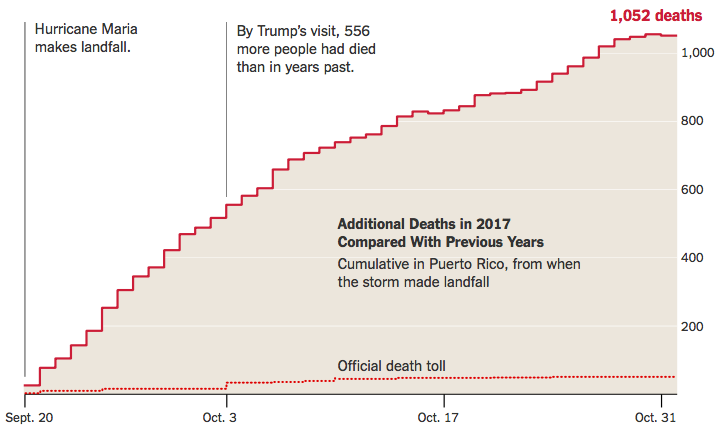
\includegraphics[width=0.9\textwidth]{figures/maria_excess_deaths.png} \end{center}

\footnotesize Source: The New York Times

\end{frame}

\begin{frame}{Counting tropical cyclone fatalities}

\begin{center}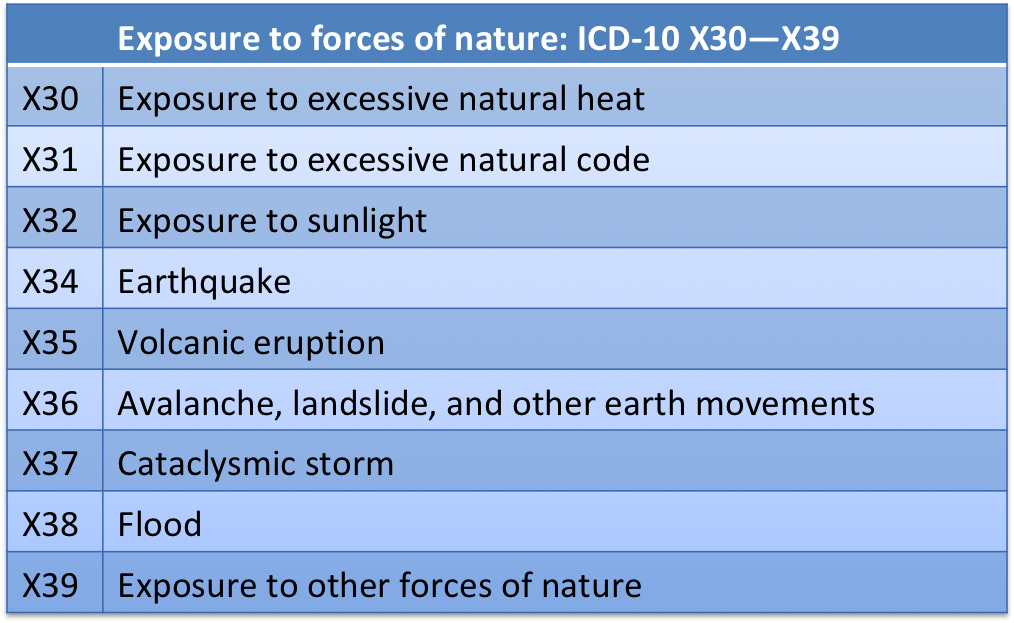
\includegraphics[width=\textwidth]{figures/icd_disaster_codes} \end{center}

\end{frame}

\begin{frame}{Reporting cause of death}

\begin{center}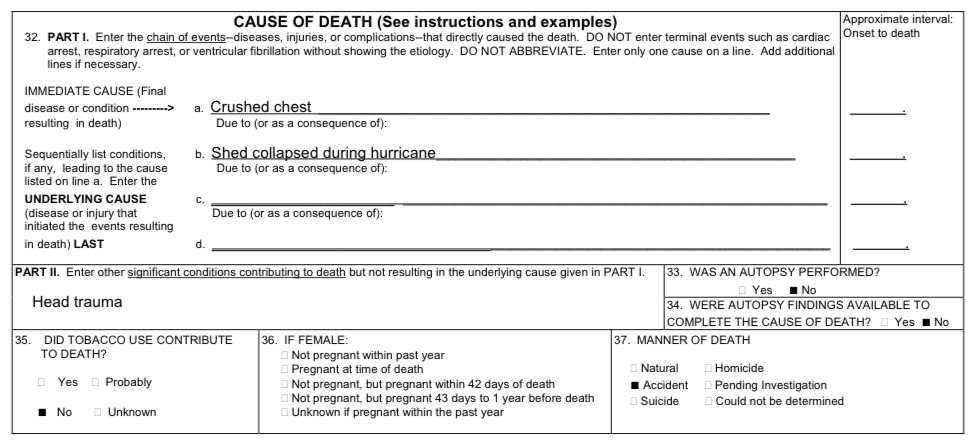
\includegraphics[width=\textwidth]{figures/cdc_direct_death} \end{center}

\footnotesize Source:
\url{https://www.cdc.gov/nchs/data/dvs/hurricane_certification.pdf}

\end{frame}

\begin{frame}{Reporting cause of death}

\begin{center}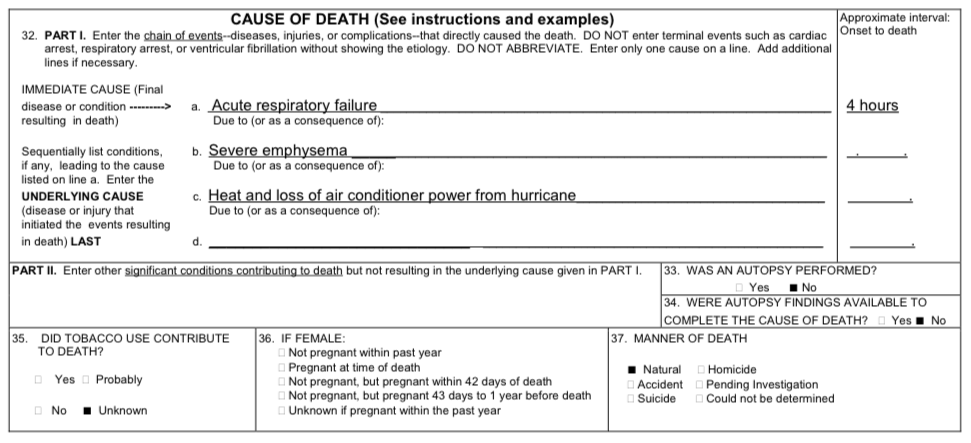
\includegraphics[width=\textwidth]{figures/cdc_indirect_death} \end{center}

\footnotesize Source:
\url{https://www.cdc.gov/nchs/data/dvs/hurricane_certification.pdf}

\end{frame}

\begin{frame}{Reporting cause of death}

\begin{center}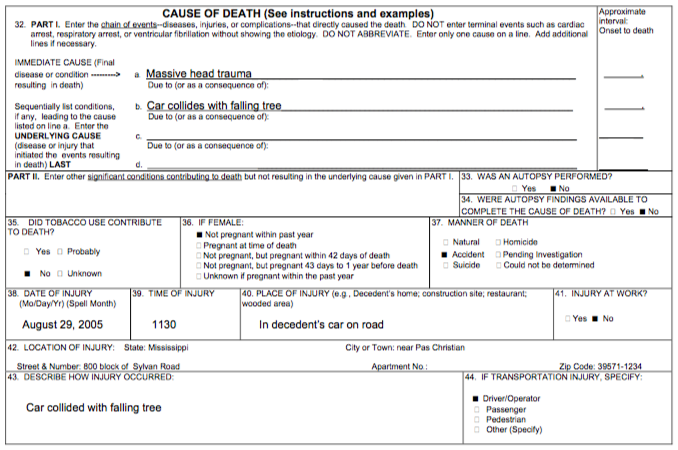
\includegraphics[width=\textwidth]{figures/cdc_notlinked_death} \end{center}

\footnotesize Source:
\url{https://www.cdc.gov/nchs/data/dvs/hurricane_certification.pdf}

\end{frame}

\begin{frame}{Impacts in excess of official death tolls}

Evidence from Hurricane Maria in Puerto Rico.

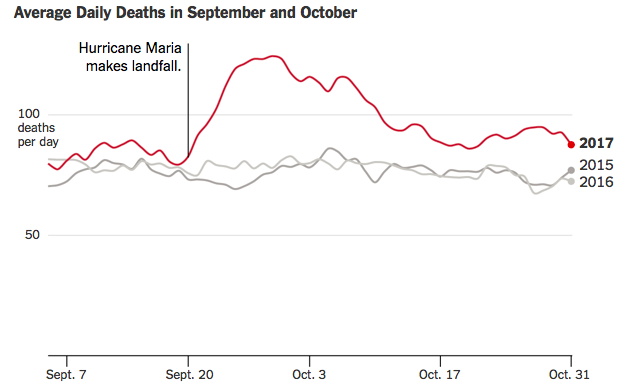
\includegraphics[width=\textwidth]{figures/maria_timeseries}

\footnotesize Source: The New York Times

\end{frame}

\begin{frame}{Relative risk of mortality associated with storm exposure}

\begin{block}{Relative risk of mortality associated with storm exposure}
We aimed to measure the \textit{relative risk (RR)} of mortality during the storm compared to what would have been expected the same days if there had not been a storm:

\begin{equation*}
RR = \frac{\text{\# deaths during storm}}{\text{Expected \# of deaths without storm}}
\end{equation*}

\end{block}

\end{frame}

\begin{frame}{Study storms and communities}

\begin{center}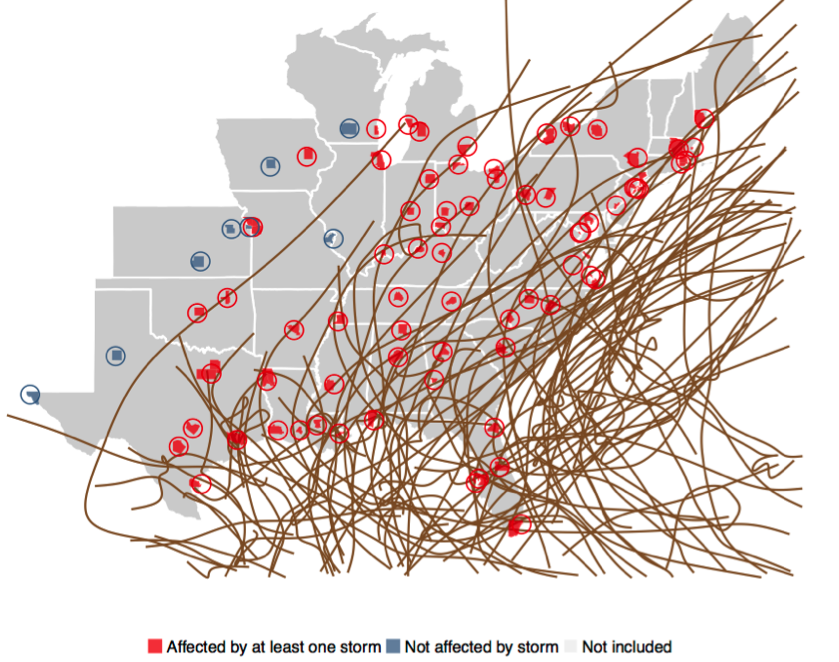
\includegraphics[width=0.85\textwidth]{figures/mortality_storms_counties} \end{center}

\footnotesize Source: Preliminary results, Yan et al.

\end{frame}

\begin{frame}{Seasonality in tropical cyclones}

Storm occurence by month for three high-risk US counties.

\begin{center}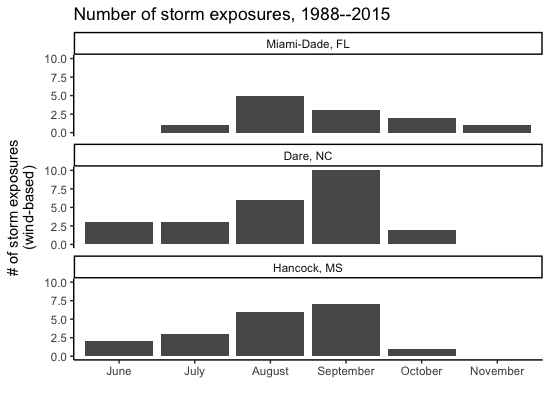
\includegraphics[width=0.8\textwidth]{figures/storm_seasonality} \end{center}

\end{frame}

\begin{frame}{Seasonal confounding}

\begin{center}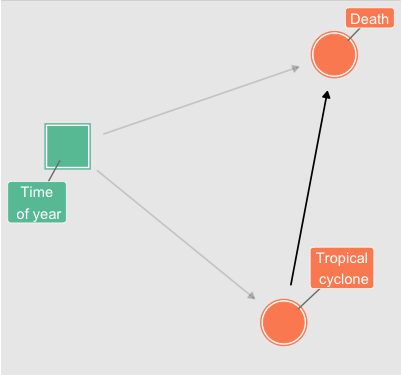
\includegraphics[width=0.6\textwidth]{figures/seasonal_confounding} \end{center}

\small The probability of both tropical storms and mortality vary by
season, opening the potential for season to confound measurements of the
relationship between tropical storm exposure and mortality risk.

\end{frame}

\begin{frame}{Matching to control for seasonality}

\begin{center}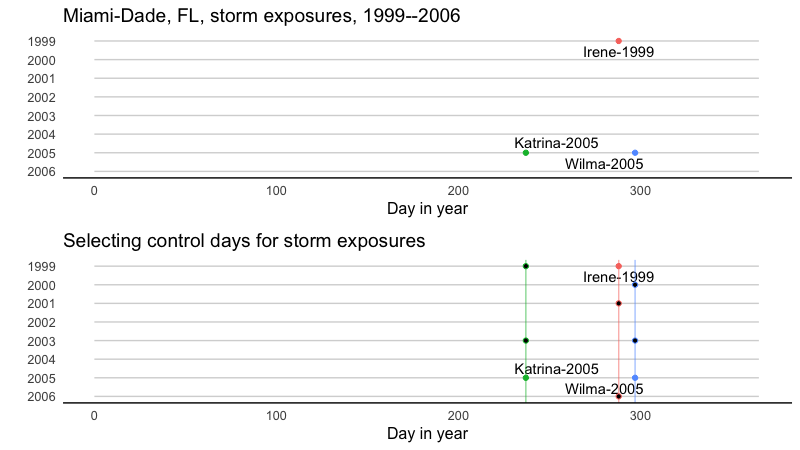
\includegraphics[width=\textwidth]{figures/example_picking_controls} \end{center}

\small We selected unexposed days in each community, matched to each
storm exposed day, ensuring all matches are on similar days of the year.

\end{frame}

\begin{frame}{Potential pathways through which tropical cyclone exposure
might increase mortality risk}

\begin{center}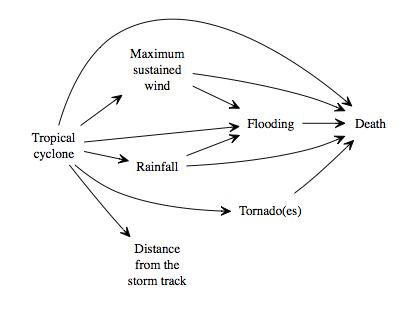
\includegraphics[width=0.9\textwidth]{figures/storm_death_pathways} \end{center}

\end{frame}

\begin{frame}{Metrics of tropical cyclone exposure used previously}

\begin{center}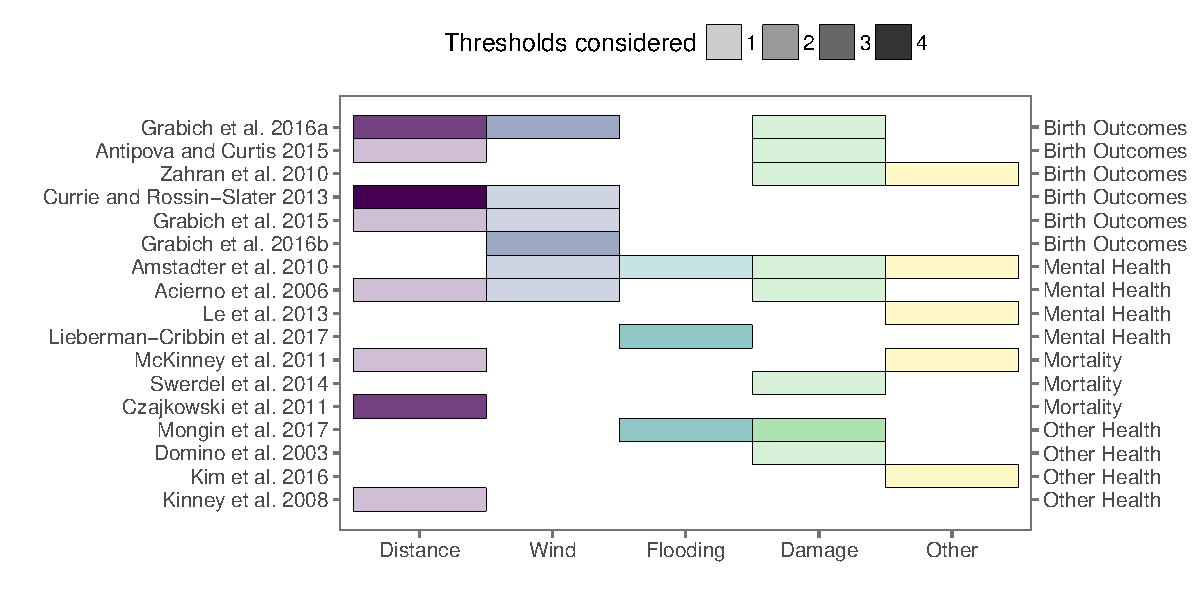
\includegraphics[width=\textwidth]{figures/previous_exposure_metrics} \end{center}

\end{frame}

\begin{frame}{Distance as a surrogate measure of tropical cyclone
exposure}

\begin{center}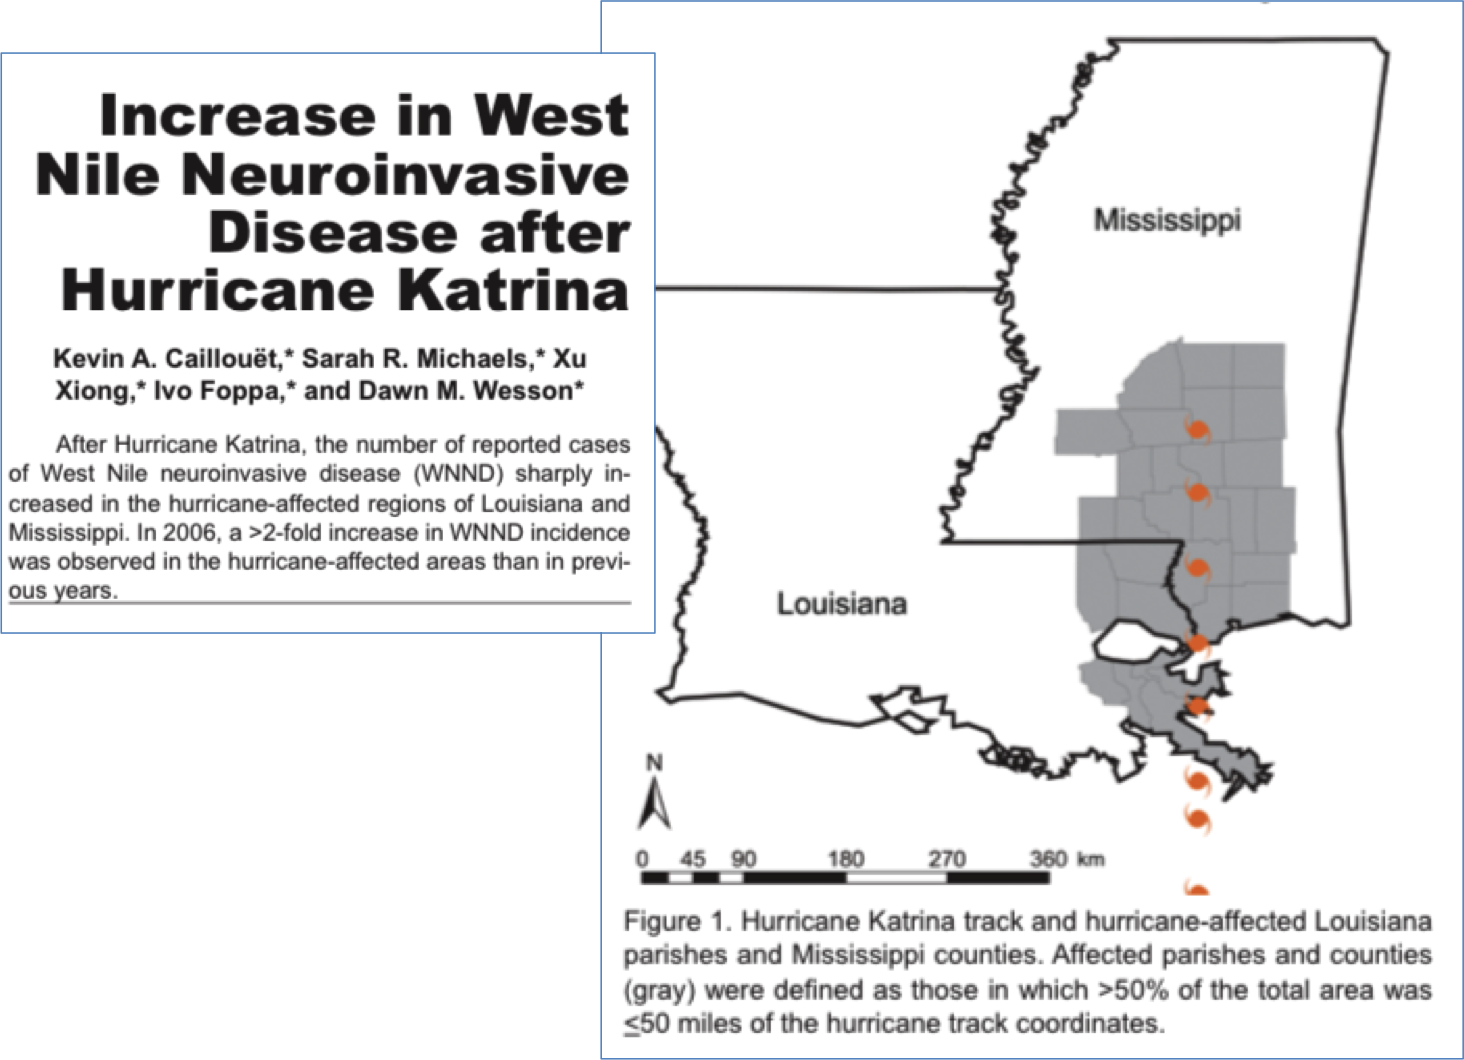
\includegraphics[width=\textwidth]{figures/katrina_west_nile} \end{center}

\end{frame}

\begin{frame}{Potential pathway for effects of Katrina on West Nile
risk}

\begin{center}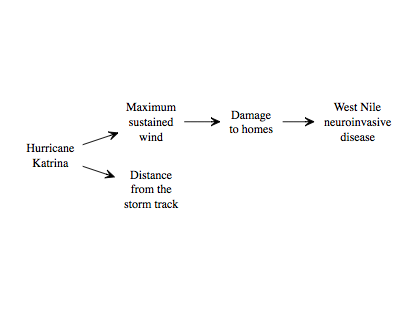
\includegraphics[width=\textwidth]{figures/causal_wind} \end{center}

\end{frame}

\begin{frame}{Katrina wind exposure vs.~distance from storm track}

\begin{center}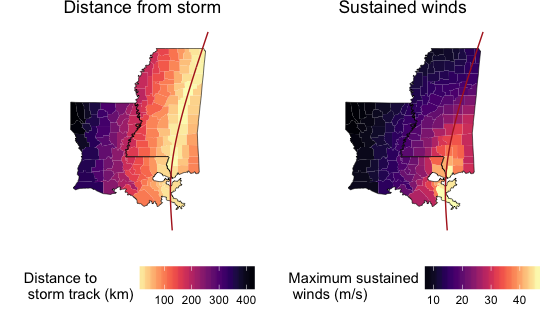
\includegraphics[width=\textwidth]{figures/katrina_continuous_exposures} \end{center}

\footnotesize For each county in Louisiana and Mississippi, we measured
the distance of the county's population mean center from the storm track
(left) and modeled the maximum sustained windspeed associated with the
storm (right).

\end{frame}

\begin{frame}{Katrina wind exposure vs.~distance from storm track}

\begin{center}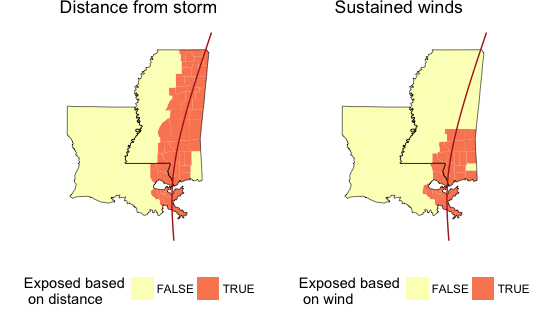
\includegraphics[width=\textwidth]{figures/katrina_exposure_discrete} \end{center}

\footnotesize Binary storm exposure classifications based on distance
from the storm track (left) and maximum sustained wind (right) for
Hurricane Katrina.

\end{frame}

\begin{frame}{Katrina wind exposure vs.~distance from storm track}

\begin{center}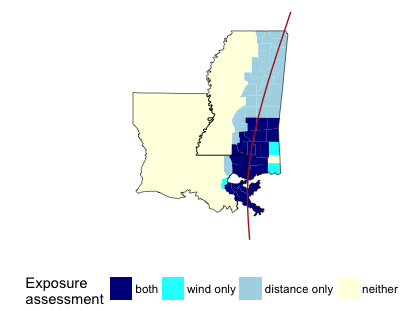
\includegraphics[width=0.8\textwidth]{figures/katrina_exposure_class} \end{center}

\footnotesize Differences between storm exposure classifications when
using distance versus maximum sustained winds.

\end{frame}

\begin{frame}{Relationships among tropical cyclone hazards}

\begin{center}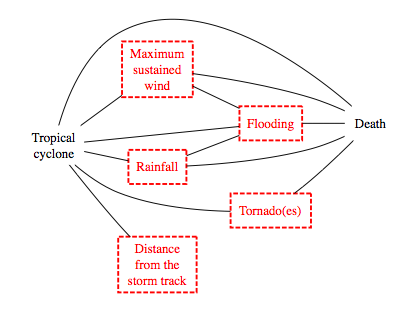
\includegraphics[width=0.8\textwidth]{figures/metric_relationships} \end{center}

\end{frame}

\begin{frame}{Tropical storm exposure classifications for Hurricane
Katrina}

\begin{center}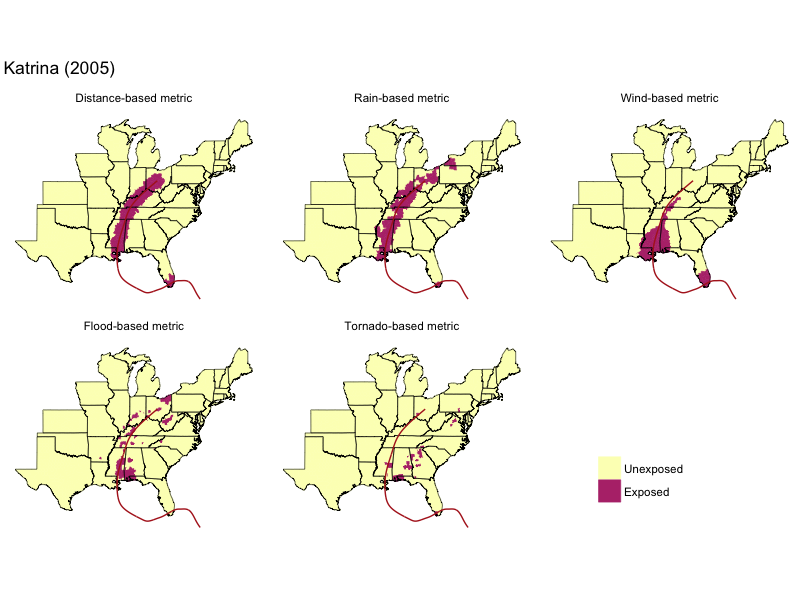
\includegraphics[width=\textwidth]{figures/katrina_all_exposures} \end{center}

\end{frame}

\begin{frame}{Similarity among tropical cyclone hazards}

\begin{center}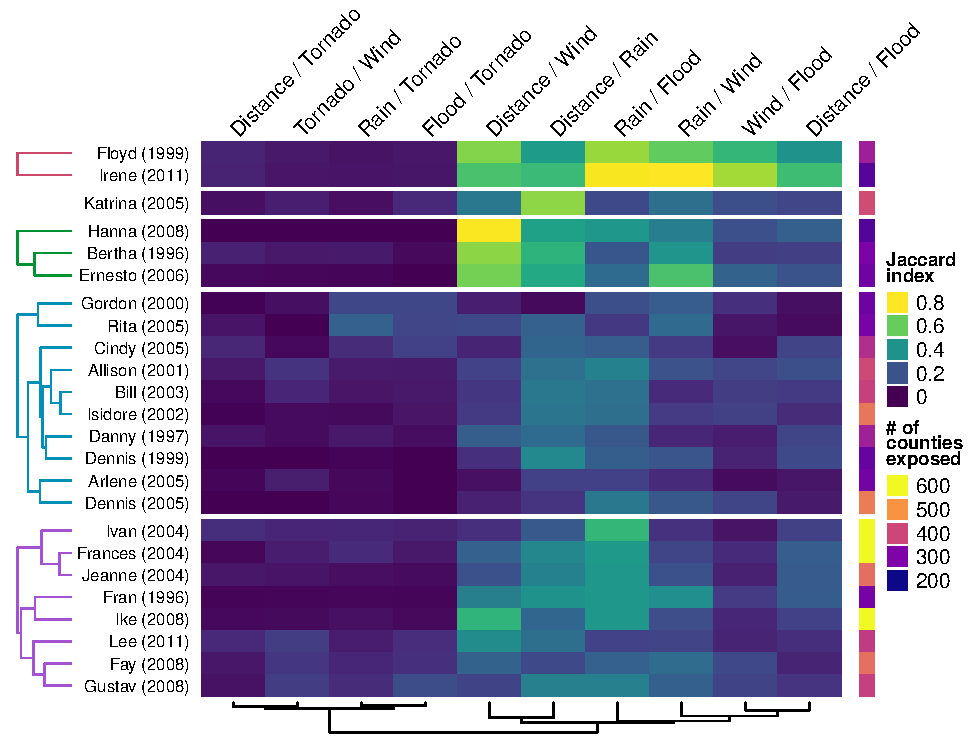
\includegraphics[width=\textwidth]{figures/jaccard_heatmap_presentation} \end{center}

\end{frame}

\begin{frame}{Associations between storm hazards and mortality}

\begin{center}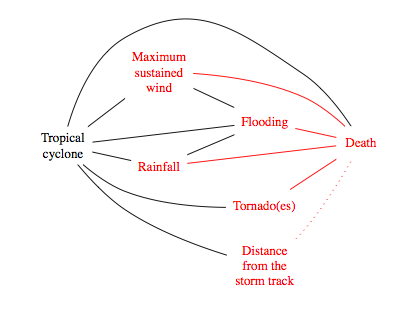
\includegraphics[width=0.8\textwidth]{figures/metric_associations_with_mortality} \end{center}

\end{frame}

\begin{frame}{Mortality risks by day during storm period}

\begin{columns}
\begin{column}{0.6\textwidth}  
    \begin{center}
     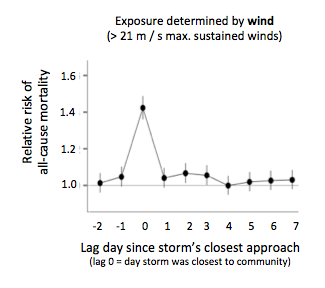
\includegraphics[width=\textwidth]{figures/all_cause_lags.png}
     \end{center}
\end{column}
\begin{column}{0.4\textwidth}
\footnotesize
\begin{block}{Risks by day}
\footnotesize
\begin{itemize}
  \item For all-cause deaths, RRs were highest on storm's closest day
  \item There was some evidence of elevated risk before and after the storm
  \item Lag patterns were similar for cardiovascular and accidental deaths
\end{itemize}
\end{block}
\end{column}
\end{columns}

\footnotesize Source: Preliminary results, Yan et al.

\end{frame}

\begin{frame}{Mortality risk by exposure metric}

\begin{center}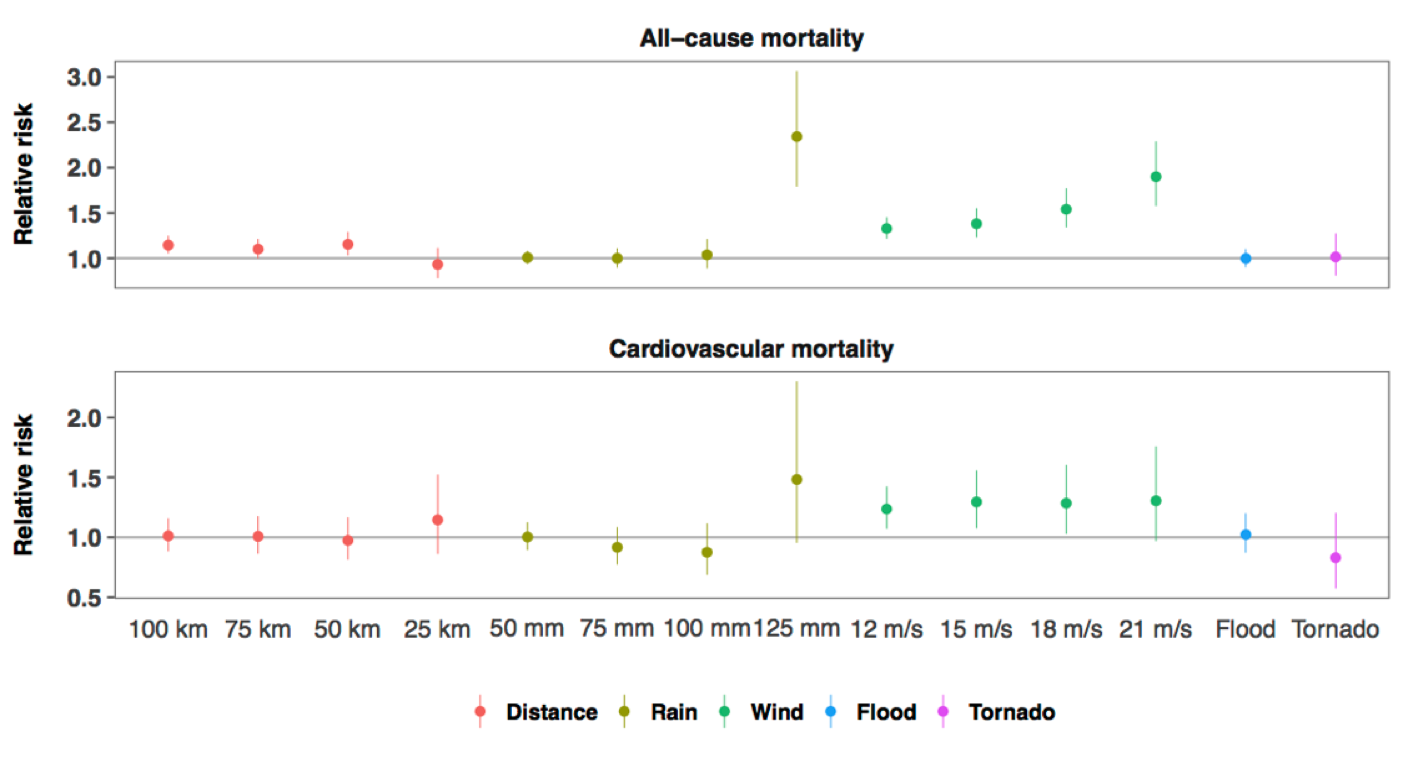
\includegraphics[width=\textwidth]{figures/rrs_by_metric} \end{center}

\footnotesize Source: Preliminary results, Yan et al.

\end{frame}

\end{document}
